\documentclass[11pt,a4paper]{article}

\usepackage[T1]{fontenc}
\usepackage[utf8]{inputenc}
\usepackage[margin=2.2cm]{geometry}
\usepackage{amsmath,amssymb}
\usepackage{xcolor}
\usepackage{listings}
\usepackage{enumitem}
\usepackage{booktabs}
\usepackage{tikz}
\usetikzlibrary{positioning,arrows.meta,shapes.geometric,fit,backgrounds,calc}
\usepackage[hidelinks]{hyperref}

% ---- inline / block code style ------------------------------------------
\definecolor{codebg}{gray}{0.96}
\definecolor{kw}{RGB}{0,90,160}
\lstset{
  basicstyle=\ttfamily\small,
  keywordstyle=\color{kw}\bfseries,
  commentstyle=\color{gray},
  columns=fullflexible,
  keepspaces=true,
  breaklines=true,
  language=Python,
  showstringspaces=false,
  backgroundcolor=\color{codebg},
  frame=none,
}
% inline code helper (robust to underscores in macro arguments)
\newcommand{\code}[1]{\texttt{\detokenize{#1}}}
% function entry: \fn{signature}{description}
\newcommand{\fn}[2]{%
  \par\smallskip\noindent\texttt{\detokenize{#1}}\\[1pt]%
  \nopagebreak\hspace*{1.2em}\begin{minipage}[t]{0.93\linewidth}\small #2\end{minipage}\par
}

\title{\textbf{Genetic Fuzzy Tree (GFT) for N-CMAPSS}\\[2pt]
\large Code documentation: \texttt{gft.py}, \texttt{ncmapss\_features.py},
\texttt{gft\_analysis.py}}
\author{}
\date{}

\begin{document}
\maketitle
\vspace{-2.2em}

\section{Overview}

The model is a \emph{nested} Genetic Fuzzy Tree (GFT) trained \textbf{end-to-end}
by a real-coded genetic algorithm (GA). It is a genuine tree, not a chain of
independent stages: small sub-FIS (each $1$--$3$ inputs $\to$ 1 output) are
composed, and the \emph{output of a child FIS is an input of its parent}.

\begin{itemize}[leftmargin=1.4em,itemsep=1pt]
\item \textbf{Leaves --- diagnosis.} One FIS per health modifier maps real
      cruise sensors to an estimated health parameter,
      \code{[sensors] -> theta_hat}. Leaves are \emph{supervised}: each has a
      $\theta$ target, so $\hat\theta$ is directly comparable to ground truth.
\item \textbf{Spool nodes --- aggregation.} \code{hp} and \code{lp} fuse the two
      modifiers of each shaft into one \emph{latent} damage value in $[0,1]$.
      They have no target of their own.
\item \textbf{Root --- prognosis.} \code{RUL(hp, lp, age)} outputs the remaining
      useful life. Also latent-in, supervised-out.
\end{itemize}

\noindent The whole genome (all nodes at once) is optimised against a single
scalar loss; the intermediate spool nodes are discovered by the GA.

\paragraph{Fuzzy model.} Each FIS is a \textbf{zero-order Takagi--Sugeno} system
on a \emph{full grid} of rules. Inputs are fuzzified with a \textbf{Ruspini
partition} (triangles that sum to 1 everywhere). With the product t-norm and the
full grid, the rule firing strengths sum to exactly~1:
\[
  \sum_{\text{rules}} \; \prod_d \mu_{d,i_d}(x_d)
  \;=\; \prod_d \Big(\sum_i \mu_{d,i}(x_d)\Big) \;=\; 1 ,
\]
so the Sugeno weighted average reduces to a plain dot product with the rule
singletons $c_r$:
\[
  y(x)=\sum_r f_r(x)\, c_r .
\]
\textbf{Antecedent centres are fixed} (data quantiles in z-space for sensors;
the target's quantiles or $[0,1]$ for node inputs). The GA therefore optimises
\emph{only the singletons} --- one scalar per grid cell --- which keeps the model
small, linear in its free parameters, and interpretable. The TSK order-1 mode,
the roughness penalty and the monotone-consequent machinery of the previous
version have been removed.

\paragraph{Hybrid loss.} A single scalar drives the whole tree:
\[
  \mathcal{L} \;=\;
  \underbrace{\mathrm{NASA}(\mathrm{RUL})}_{\text{prognosis}}
  \;+\;
  w_\theta \cdot \underbrace{\frac{1}{L}\sum_{\ell}
     \frac{\mathrm{RMSE}(\hat\theta_\ell,\theta_\ell)}{\mathrm{range}(\theta_\ell)}}_{\text{magnitude}}
  \;+\;
  w_{\mathrm{tr}} \cdot \underbrace{\frac{1}{L}\sum_{\ell}
     \operatorname*{mean}_{u\in\text{units}}\!\big(1-\rho(\hat\theta_\ell,\theta_\ell)\big|_u\big)}_{\text{trend / shape}}
\]
Both $\theta$ terms are \textbf{scale-free}: the magnitude term is divided by the
target range, and the trend term is a Pearson correlation $\rho$ computed
\emph{per unit}. Consequently, multiplying the sensors or the $\theta$ targets by
any constant leaves the fit bit-identical (inputs are z-scored per node; the
consequent box and the GA's mutation step are both relative to the target range).
The trend term exists because the plain RMSE is dominated by the per-cycle noise
floor of a memoryless FIS and is therefore rather insensitive to whether the
\emph{shape} of the degradation is captured; $w_{\mathrm{tr}}\!\sim\!0.5$--$1.0$
rewards $\hat\theta$ \emph{moving with} the truth regardless of scale.

\paragraph{Real sensors only.} Only the measured sensors of C-MAPSS Table~2
($x_s$: \code{Wf Nf Nc T24 T30 T48 T50 P15 P21 P24 Ps30 P40 P50}) are used.
The virtual sensors of Table~3 ($x_v$: \code{T40 P30 P45 W* epr Sm* NR* PCNfR
phi}) are not even loaded from the \code{.h5} file.

\section{Complete GFT tree}

\begin{center}
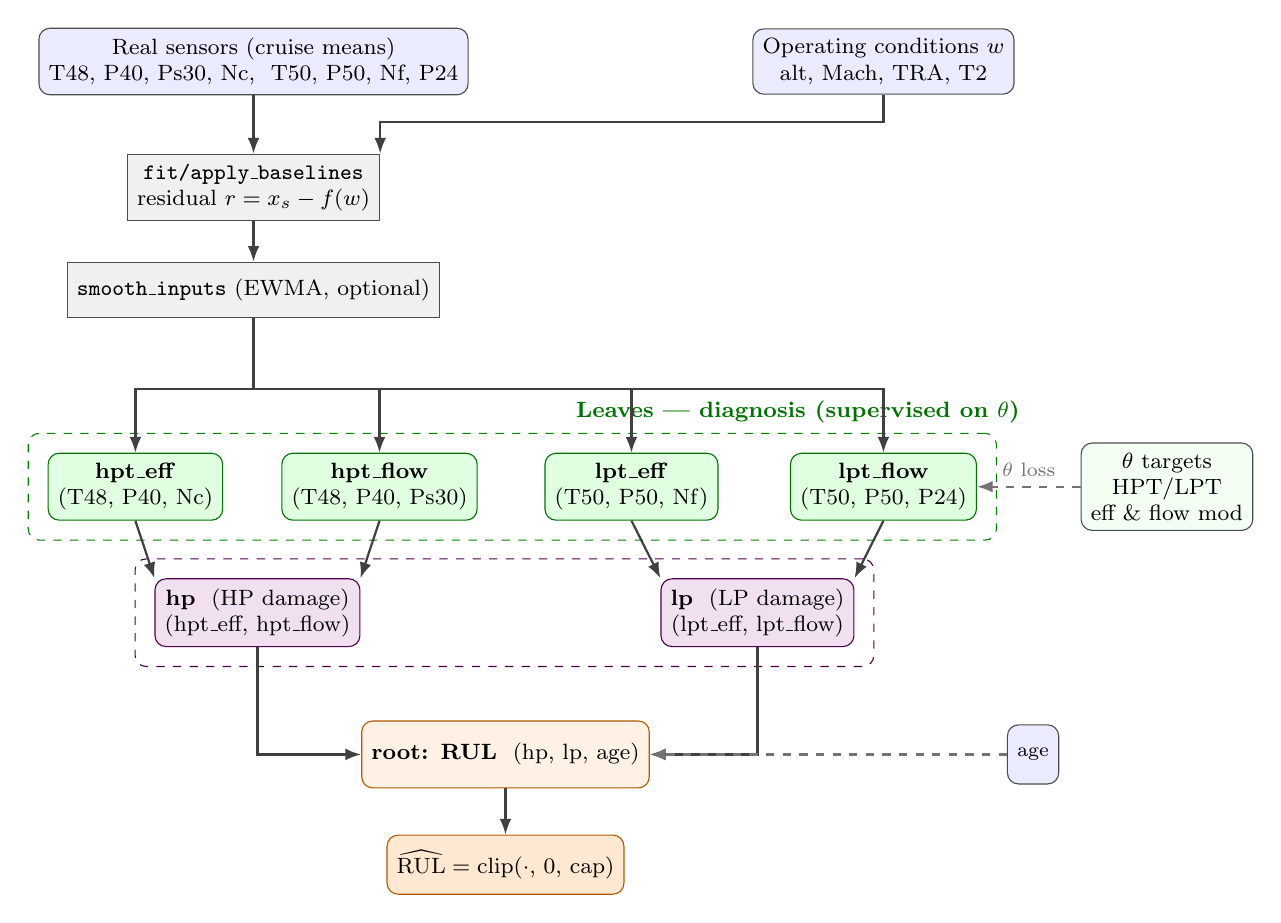
\begin{tikzpicture}[
  io/.style={rectangle, rounded corners, draw=black!70, fill=blue!8,
             align=center, inner sep=3.5pt, font=\footnotesize, minimum height=0.75cm},
  proc/.style={rectangle, draw=black!70, fill=gray!12,
             align=center, inner sep=3.5pt, font=\footnotesize, minimum height=0.7cm},
  fis/.style={rectangle, rounded corners, draw=green!45!black, fill=green!12,
             align=center, inner sep=3.5pt, font=\footnotesize, minimum height=0.85cm},
  spool/.style={rectangle, rounded corners, draw=violet!60!black, fill=violet!12,
             align=center, inner sep=3.5pt, font=\footnotesize, minimum height=0.8cm},
  outb/.style={rectangle, rounded corners, draw=orange!70!black, fill=orange!18,
             align=center, inner sep=3.5pt, font=\footnotesize, minimum height=0.75cm},
  arr/.style={-{Latex[length=2mm]}, thick, black!75},
  darr/.style={-{Latex[length=2mm]}, thick, dashed, black!55},
]

% --- inputs ---
\node[io] (sens) at (0,0) {Real sensors (cruise means)\\ T48, P40, Ps30, Nc,\ \ T50, P50, Nf, P24};
\node[io] (w)    at (8.0,0) {Operating conditions $w$\\ alt, Mach, TRA, T2};

% --- preprocessing ---
\node[proc] (resid)  at (0,-1.6) {\texttt{fit/apply\_baselines}\\ residual $r=x_s-f(w)$};
\node[proc] (smooth) at (0,-2.9) {\texttt{smooth\_inputs} (EWMA, optional)};

% --- leaves : four supervised sub-FIS ---
\node[fis] (f1) at (-1.5,-5.4) {\textbf{hpt\_eff}\\ (T48, P40, Nc)};
\node[fis] (f2) at ( 1.6,-5.4) {\textbf{hpt\_flow}\\ (T48, P40, Ps30)};
\node[fis] (f3) at ( 4.8,-5.4) {\textbf{lpt\_eff}\\ (T50, P50, Nf)};
\node[fis] (f4) at ( 8.0,-5.4) {\textbf{lpt\_flow}\\ (T50, P50, P24)};

% theta targets (supervision)
\node[io, fill=green!5] (th) at (11.6,-5.4)
  {$\theta$ targets\\ \footnotesize HPT/LPT\\ \footnotesize eff \& flow mod};

% --- spool nodes ---
\node[spool] (hp) at (0.05,-7.0) {\textbf{hp}\ \ (HP damage)\\ (hpt\_eff, hpt\_flow)};
\node[spool] (lp) at (6.4,-7.0) {\textbf{lp}\ \ (LP damage)\\ (lpt\_eff, lpt\_flow)};

% --- root ---
\node[fis, draw=orange!70!black, fill=orange!10] (rul) at (3.2,-8.8)
  {\textbf{root: RUL}\ \ (hp, lp, age)};
\node[outb] (out) at (3.2,-10.2) {$\widehat{\mathrm{RUL}}=\mathrm{clip}(\cdot,\,0,\,\text{cap})$};

% --- arrows ---
\draw[arr] (sens) -- (resid);
\draw[arr] (w.south) -- ++(0,-0.35) -| (resid.north east);
\draw[arr] (resid) -- (smooth);
\draw[arr] (smooth.south) -- ++(0,-0.9) -| (f1.north);
\draw[arr] (smooth.south) -- ++(0,-0.9) -| (f2.north);
\draw[arr] (smooth.south) -- ++(0,-0.9) -| (f3.north);
\draw[arr] (smooth.south) -- ++(0,-0.9) -| (f4.north);
\draw[arr] (f1.south) -- (hp.north west);
\draw[arr] (f2.south) -- (hp.north east);
\draw[arr] (f3.south) -- (lp.north west);
\draw[arr] (f4.south) -- (lp.north east);
\draw[arr] (hp.south) |- ($(rul.west)+(-0.0,0)$);
\draw[arr] (lp.south) |- ($(rul.east)+(0.0,0)$);
\draw[arr] (rul) -- (out);
% supervision of the leaves (dashed)
\draw[darr] (th.west) -- (f4.east)
      node[pos=0.5,above,font=\scriptsize]{$\theta$ loss};
% age into the root
\node[io,font=\scriptsize] (age) at (9.9,-8.8) {age};
\draw[darr] (age.west) -- (rul.east);

% --- containers ---
\begin{scope}[on background layer]
  \node[draw=green!50!black, dashed, rounded corners, inner sep=7pt,
        fit=(f1)(f2)(f3)(f4),
        label={[green!45!black,font=\footnotesize\bfseries]above right:{Leaves --- diagnosis (supervised on $\theta$)}}] {};
  \node[draw=violet!60!black, dashed, rounded corners, inner sep=7pt,
        fit=(hp)(lp),
        label={[violet!55!black,font=\footnotesize\bfseries]above:{}}] {};
\end{scope}

\end{tikzpicture}
\end{center}

\noindent\emph{How to read it.} The real sensors are first stripped of the
dominant flight-condition effect ($x_s-f(w)$), optionally EWMA-smoothed along
cycles, then fed to the four leaf FIS. Each leaf predicts one health modifier and
is pulled by the $\theta$ loss. The two \emph{latent} spool nodes fuse
(\code{eff}, \code{flow}) into a single damage value per shaft, and the root FIS
turns (\code{hp}, \code{lp}, \code{age}) into RUL. The tree is \textbf{symmetric
by construction}: each shaft (HP $=$ HPT; LP $=$ Fan/LPC/LPT) has an efficiency
leaf and a flow leaf feeding a global shaft-damage node. In DS02, \code{HPT\_flow}
happens to be constant; its leaf then simply predicts that constant (the tight
consequent box keeps it noise-free), and the same tree still works on failure
modes where HPT flow does move.

\paragraph{Editing the topology.} The tree is a single module constant,
\code{TREE}: a list of \code{(name, [inputs], theta_target_or_None)}. An input is
either a data column (a sensor, or \code{"age"}) or the name of an earlier node.
Children must precede parents, the root must be named \code{"RUL"}, and a node
takes at most 3 inputs. Per-input membership counts are given by writing an input
as a pair:

\begin{lstlisting}
TREE = [
    ("hpt_eff",  [("T48", 5), ("P40", 3), "Nc"], "HPT_eff_mod"),  # T48 -> 5 sets
    ("hpt_flow", ["T48", "P40", "Ps30"],         "HPT_flow_mod"),
    ("lpt_eff",  ["T50", "P50", "Nf"],           "LPT_eff_mod"),
    ("lpt_flow", ["T50", "P50", "P24"],          "LPT_flow_mod"),
    ("hp",  [("hpt_eff", 2), ("hpt_flow", 2)], None),
    ("lp",  ["lpt_eff", "lpt_flow"],           None),
    ("RUL", ["hp", "lp", ("age", 6)],          None),
]
\end{lstlisting}

\noindent A bare name uses the default \code{n_terms}. A node's rule count is the
\emph{product} of its inputs' set counts, so $(5,3,3)\Rightarrow 45$ rules --- and
45 GA parameters for that node alone. Only put a $\theta$ target on a modifier
that actually moves.

\section{Reference: \texttt{gft.py}}

\subsection*{1. Fuzzy inference}
\fn{_centers(x, n)}{$n$ ordered Ruspini set-centres for one variable, placed at
data quantiles so the fuzzy sets are populated. Guards against ties and
near-constant inputs.}
\fn{_memberships(x, c)}{Triangular memberships, an
$(n_\text{samples}\times n_\text{terms})$ matrix whose rows sum to~1. Each set is
the piecewise-linear hat $0\!\to\!1\!\to\!0$; the two end sets are shouldered
(flat~1 beyond the extreme centres), obtained for free by clamping in
\code{np.interp}.}
\fn{_fis(cols, centers, singletons)}{One FIS: product t-norm firing over the full
grid (C-order), then the Sugeno weighted average. The division by
$\sum$\,firing is a no-op under a Ruspini partition but stays safe if a centre
set degenerates.}

\subsection*{2. Tree construction}
\fn{_parse_input(inp, default)}{\code{("name", k)} $\to$ \code{(name, k)};
a bare \code{"name"} $\to$ \code{(name, default)}. This is what enables per-input
membership counts.}
\fn{_leaf_sensors(tree)}{Sorted, de-duplicated list of the data columns the tree
reads (i.e. everything that is not a node name and not \code{"age"}).}
\fn{_domain_centers(dom, k)}{$k$ centres over a child node's output domain: the
$\theta$ quantiles for a supervised leaf, $[0,1]$ for a latent node. Lets a parent
partition a child's output at its own resolution.}
\fn{build_tree(frame, tree=TREE, n_terms=3)}{Resolve every node's inputs against
\code{frame} and \emph{fix} the fuzzy centres (sensors: quantiles of the z-scored
column, storing \code{mu}/\code{sd}; node inputs: the child's output domain).
Inputs absent from the frame are silently dropped. Returns \code{meta}, a list of
plain dicts \code{{name, inputs, n_rules, target, root}} --- there is no
\code{FISNode} class.}
\fn{n_params(meta)}{Total number of GA parameters (the sum of the nodes' rule
counts, since only the singletons are free).}
\fn{genome_bounds(meta, frame, rul_hi, cons_pad=0.25)}{Per-node singleton box: the
$\theta$ data range $\pm\,$\code{cons_pad}$\cdot$span for a supervised leaf,
$[0,1]$ for a latent spool node, $[0,\code{rul_hi}]$ for the root. A
\textbf{(near-)constant target} gets a \emph{tight} box around its mean instead
of an inflated default --- this is what stops a flat modifier (e.g.
\code{HPT_flow} in DS02) from being filled with GA noise.}
\fn{predict_tree(frame, meta, genome)}{Evaluate the whole tree in topological
order; returns \code{{node_name: output_array}}. Latent nodes are clipped to
$[0,1]$; leaves and the root are left on their natural scale.}

\subsection*{3. Losses}
\fn{rmse(a, b)}{Root-mean-square error.}
\fn{nasa_score(y_true, y_pred)}{Asymmetric NASA/PHM prognostics score. Late
predictions ($d>0$, dangerous) are penalised harder ($/10$) than early ones
($d<0$, safe, $/13$); zero at a perfect prediction. Minimising it makes the model
prefer to under-predict RUL.}
\fn{_pearson(a, b)}{Pearson correlation; returns 0 if either series is
(near-)constant.}
\fn{trend_penalty(pred, truth, unit_groups)}{Mean over units of
$1-\rho(\hat\theta,\theta)$ across that unit's cycles. \emph{Scale-free} and
noise-robust: it rewards $\hat\theta$ \textbf{moving with} the truth rather than
matching its magnitude. Units whose true $\theta$ is constant carry no trend and
are skipped; a flat prediction against a moving truth scores $\rho=0$, i.e. the
full penalty~1.}

\subsection*{4. Genetic algorithm}
\fn{_tournament(fit, rng)}{Tournament selection, $k=3$.}
\fn{genetic_optimize(loss, lo, hi, pop=80, gens=120, seed=0, x0=None, verbose=True, label="")}{Minimise
\code{loss(genome)} over the box $[\text{lo},\text{hi}]$. Tournament selection,
BLX-$\alpha$ crossover, Gaussian mutation, elitism (2), and a geometrically
cooling mutation step $\sigma$ (floored at 0.05). Optionally seeded at \code{x0}.
Returns (best genome, history).}

\subsection*{5. Condition residuals and smoothing}
\fn{_design(frame, conds)}{Design matrix $[1,\ w,\ w^2]$ for the available
operating conditions.}
\fn{_healthy_mask(frame)}{Rows to fit the healthy baseline on: pre-onset cycles
if \code{since_onset} is known, otherwise each unit's first half of life.}
\fn{fit_baselines(frame, sensors, conds)}{Least-squares baseline coefficients per
sensor, fit on healthy rows.}
\fn{apply_baselines(frame, coefs, conds)}{Replace each sensor by its residual
$x_s-f(w)$ (in place, same column name). This strips the dominant
flight-condition effect that would otherwise bury the small degradation term.}
\fn{smooth_inputs(frame, cols, span)}{EWMA-smooth the sensor columns along cycles
\emph{within} each unit; \code{span<=1} is a no-op. The FIS is \emph{memoryless},
so per-cycle sensor noise passes straight into $\hat\theta$; smoothing the inputs
here (identically at fit and predict time) is the direct cure for the
cycle-to-cycle jitter.}

\subsection*{6. Fit / predict}
\fn{fit_gft(frame, tree=TREE, n_terms=3, pop=80, gens=120, residualize=True, smooth_span=0, rul_cap=None, theta_weight=1.0, trend_weight=0.0, seed=0, verbose=True)}{Train
the \emph{whole} tree end-to-end on the hybrid loss of \S1: NASA score on RUL,
plus \code{theta_weight}$\,\times\,$the range-normalised $\theta$ RMSE, plus
\code{trend_weight}$\,\times\,$the per-unit correlation penalty.
\code{theta_weight=0} recovers pure RUL training; \code{trend_weight}
$\sim0.5$--$1.0$ sharpens trend fidelity. \code{rul_cap} applies the piecewise-linear
(capped) RUL convention. Returns a plain-dict model (\code{tree}, \code{meta},
\code{genome}, \code{history}, \code{baselines}, \code{conds}, and the config
echoes).}
\fn{predict_gft(frame, model)}{Full inference: sensors $\to\hat\theta\to$
(\code{hp}, \code{lp}) $\to$ RUL. Applies the same residualisation and smoothing
as at fit time. Returns a frame with \code{unit}, \code{cycle}, one
\code{<THETA>_hat} column per supervised leaf, one \code{<node>_h} column per
latent node, and \code{RUL_hat} (clipped to $[0,\code{rul_cap}]$).}
\fn{inspect(model)}{Print, per FIS: its inputs, its target, its grid shape and the
range of its learned singletons.}

\subsection*{7. Self-test}
\fn{_synthetic_frame(units, cycles, seed)}{Signal-bearing synthetic frame in the
extractor's schema: $\theta$ drifting after an onset, a per-flight operating
point, real-sensor columns carrying a large condition effect plus a small damage
effect, RUL $=$ EOL $-$ cycle.}
\fn{_self_test()}{Check the Ruspini partition of unity, train on the synthetic
frame and print the train/test $\theta$ and RUL RMSEs against a mean baseline.}

\medskip
\noindent\textbf{Module constants.} \code{TREE} (the topology; see \S2) and
\code{CONDITIONS} (the operating conditions used for the healthy baseline).

\section{Reference: \texttt{ncmapss\_features.py}}

Turns an N-CMAPSS \code{.h5} file into \emph{one row per (unit, cycle)}. Because
$\theta$ is imposed once per flight (constant within a cycle at 1\,Hz), every
feature is a cruise-mean aggregated to the cycle level. Columns keep their plain
physical names (\code{T48}, \code{P40}, \dots) so the tree can reference sensors
directly.

\fn{_names(arr)}{Decode a \code{*_var} group (byte-strings, possibly 2-D) into a
flat list of clean Python strings.}
\fn{load_raw(path, split="dev")}{Load one split into a per-timestamp (1\,Hz)
DataFrame: \code{A} (unit, cycle, Fc, hs), \code{W} (conditions), \code{X_s} (real
sensors), \code{T} ($\theta$) and \code{Y} (RUL). \textbf{The virtual-sensor group
\code{X_v} is deliberately not loaded}, so no virtual sensor can reach the model
(and the real 5.3\,M-row file uses less memory).}
\fn{cycle_features(path, split="dev", cruise_frac=0.95, min_cruise=30)}{The whole
extractor. Keeps the high-altitude (cruise) part of each cycle
(\code{alt >= cruise_frac * max(alt)}), averages the sensors and conditions over
it, and returns one row per (unit, cycle) with: \code{unit}, \code{cycle},
\code{age} (1-indexed cycle count per unit), \code{since_onset} (cycles since the
health flag \code{hs} flipped $0\!\to\!1$), \code{RUL}, the four operating
conditions, the 13 real sensors and the $\theta$ modifiers. Cycles with fewer than
\code{min_cruise} cruise samples are dropped.}
\fn{_make_synthetic_h5(path, ...) / _self_test()}{Build a small N-CMAPSS-like
\code{.h5} (both \code{dev} and \code{test} groups) so the pipeline is testable
without the real file.}

\medskip
\noindent\textbf{Module constants.} \code{CONDITIONS}; \code{SENSORS} --- the 13
\emph{real} measurements of Table~2 only; \code{THETA} --- the health modifiers
kept as targets.

\section{Reference: \texttt{gft\_analysis.py}}

\subsection*{1. Utilities}
\fn{_color(u) / _grid(n)}{Per-unit colour (20-colour palette) and a compact
subplot grid.}
\fn{_slice(meta, genome, node)}{The genome slice (the singletons) belonging to one
node.}
\fn{_finish(fig, save, name, show)}{Save and/or display a figure, then close it.}
\fn{_prepare_dir(folder, clear=True)}{Create \code{folder} if it does not exist and
\textbf{wipe the existing \code{.png}} so a rerun replaces stale figures instead of
leaving orphans. Returns the filename prefix used by \code{_finish}.}

\subsection*{2. Metrics and time-series plots}
\fn{print_metrics(feats, pred)}{Per-unit RUL RMSE and NASA score, plus an
``ALL'' row.}
\fn{plot_theta(feats, pred, ...)}{\textbf{One figure per modifier}: predicted vs
actual $\theta$ against cycle, solid = real, dashed = predicted, one colour per
unit, with that modifier's RMSE in the title. This is the mid-node sanity check.}
\fn{plot_nodes(pred, ...)}{The \emph{latent} spool health (\code{hp_h},
\code{lp_h}) vs cycle, one subplot per node, $y$ clamped to $[0,1]$.}
\fn{plot_rul(feats, pred, ...)}{RUL vs cycle, one subplot per unit: real (line) vs
predicted (markers).}
\fn{plot_scatter(feats, pred, ...)}{Predicted vs true RUL, coloured per unit, with
the $y=x$ line and the global RMSE in the title.}
\fn{plot_fitness(model, ...)}{The GA training curve: best loss per generation
(single curve --- the tree is trained in one pass, not per stage).}

\subsection*{3. Control surfaces}
\fn{_disp_range(inp) / _disp_axis_centers(inp)}{Axis range and rule-grid centres in
\emph{display} units: raw (de-standardised) for sensors, native for
$\theta$/$[0,1]$ node inputs.}
\fn{_eval_disp(node, Xdisp, singletons)}{Evaluate one sub-FIS at display-unit
points, standardising internally where required.}
\fn{_surface(node, singletons, ix, iy, res=45)}{Dense $(XX,YY,ZZ)$ evaluation grid
of a sub-FIS over inputs $(ix,iy)$, any other input frozen at the centre of its
range.}
\fn{plot_surface_node(node, singletons, kind="surface", res=45, ...)}{\textbf{One
figure for one sub-FIS}: a 1-D curve for a 1-input FIS, otherwise one panel per
input \emph{pair} (1 panel for 2 inputs, 3 for 3 inputs) side by side.
\code{kind}~$\in\{$\code{"surface"} (3-D), \code{"contour"} (top-down with the
fuzzy-rule grid overlaid)$\}$.}
\fn{plot_surfaces(model, kind="surface", ...)}{Draw \emph{every} sub-FIS, each as
its own figure (\code{surface_<node>.png}) --- one giant grid of all nodes was
unreadable.}

\subsection*{4. Entry points}
\fn{analyze(feats, pred, model=None, surfaces=False, surface_kind="surface", savedir=None, show=True)}{Print
the metrics and draw every figure in one call. If \code{savedir} is given, all
figures are written to that folder (created if needed, existing \code{.png}
replaced). Passing \code{model} also plots the GA curve and, with
\code{surfaces=True}, the control surfaces.}
\fn{save_figures(feats, pred, model=None, folder="figures", surfaces=True, surface_kind="contour")}{Save
every figure into \code{folder} with no on-screen display.}

\section{Typical usage}

\begin{lstlisting}
from ncmapss_features import cycle_features
from gft import fit_gft, predict_gft, inspect
from gft_analysis import analyze

feats = cycle_features("N-CMAPSS_DS02-006.h5", split="dev")

model = fit_gft(feats, gens=200,
                residualize=True,   # strip the flight-condition effect
                smooth_span=7,      # EWMA the sensors -> tames theta jitter
                theta_weight=1.0,   # magnitude term on theta
                trend_weight=0.8)   # shape term: reward tracking the trend
pred = predict_gft(feats, model)

analyze(feats, pred, model=model, surfaces=True, surface_kind="contour",
        savedir="figures")          # one fig per theta, one per sub-FIS
inspect(model)
\end{lstlisting}

\paragraph{Tuning notes.}
\begin{itemize}[leftmargin=1.4em,itemsep=1pt]
\item \textbf{Scaling the sensors or $\theta$ does nothing.} Inputs are z-scored
      per node and both $\theta$ loss terms are relative, so a $\times100$ is a
      no-op (verified bit-identical). To make the loss more sensitive to a missed
      trend, raise \code{trend_weight}, not the units.
\item \textbf{$\hat\theta$ jitter} is structural (the FIS is memoryless), not a
      lack of training: raise \code{smooth_span} rather than \code{gens}.
\item \textbf{Rule-count blow-up:} a node's parameters $=\prod_d$(sets per input).
      Raise the per-input count only on inputs that carry real nonlinearity.
\end{itemize}

\vspace{0.6em}
\hrule
\vspace{0.4em}
\noindent\footnotesize Functions prefixed with an underscore (\texttt{\_...})
are internal; the others form each module's public API.

\end{document}